% =====================================================================================================================
% main.tex: single-file IEEE conference paper for Overleaf (IEEEtran; no external .bib, figures drawn in TikZ/pgfplots).
% Merged 2026-11-07 from the author's design draft and the evaluation workspace; real-LLM pilot added 2026-11-08. Every experimental number is read from
% a stored run in C:\Users\sunny\MEDICAL_RAG_RESEARCH_EVALUATION\04_TEST_RUNS (run IDs in captions). References were
% checked on 2026-11-07 against CrossRef, PubMed, arXiv, the NeurIPS proceedings and the USENIX Security 2025 page.
% Author block: completed 2026-11-08 (check co-authors and e-mail).
% =====================================================================================================================
\documentclass[conference]{IEEEtran}
\IEEEoverridecommandlockouts

\usepackage{cite}
\usepackage{amsmath,amssymb,amsfonts}
\usepackage{graphicx}
\usepackage{textcomp}
\usepackage{xcolor}
\usepackage{booktabs}
\usepackage{array}
\newcolumntype{L}[1]{>{\raggedright\arraybackslash}p{#1}}
\newcolumntype{C}[1]{>{\centering\arraybackslash}p{#1}}
\usepackage{url}
\usepackage{algorithm}
\usepackage{algpseudocode}
\usepackage{tikz}
\usetikzlibrary{positioning,arrows.meta,fit,backgrounds,shapes.geometric,calc,patterns}
\usepackage{pgfplots}
\pgfplotsset{compat=1.18}
\usepgfplotslibrary{groupplots}
\usepackage[hidelinks]{hyperref}

\begin{document}

\title{Adaptive Trust-Aware Retrieval-Augmented Generation for Medical Evidence: Guarding Against Prompt Injection
and Retrieval-Induced Hallucination}

% Author details from the author's profile (2026-11-08). Add co-authors (e.g. the faculty guide) here if any.
\author{\IEEEauthorblockN{Sandeep Sunny Mummuluri}
\IEEEauthorblockA{Department of Computing Technologies, College of Engineering and Technology\\
SRM Institute of Science and Technology, Kattankulathur, Chennai, India\\
sunnysandeep9999@gmail.com}}

\maketitle

\begin{abstract}
Retrieval-augmented generation (RAG) lets a large language model (LLM) draw on external documents, but retrieval does not
make evidence reliable. A medical retriever can return passages that are irrelevant, outdated, attached to the wrong
drug, or written to manipulate the model, and a conventional pipeline treats all of them alike once they reach the
context window. We built a trust-aware RAG prototype for drug-drug interaction (DDI) and adverse drug event (ADE)
questions that holds every retrieved item as untrusted data. Before generation, a chunk is excluded if its provenance
check fails, its content hash does not match, it carries instructions addressed to the model, it names none of the
requested medications, or its source identity is unverified; the remaining chunks must reach a risk-tiered trust
threshold. After generation, each claim is checked by a pinned natural-language-inference (NLI) model at clause level,
by a drug-pair identity check, by citation checks and by a medication identity gate, and a claim is released only when
all of them agree. We report an offline engineering evaluation. The frozen candidate reproduced byte for byte, with
2{,}252 backend tests passing in normal and network-blocked modes. On a constructed, author-known set of 113 statements,
the identity gate passed none of 54 unsupported statements (95\% upper bound 6.6\%) and wrongly withheld 2 of 59 valid
ones; across seven development sets no unsupported statement was released, and recomputing the release decision from
the recorded checks showed that without the identity gate the other checks would have released 3 to 19
identity-unsupported statements per set. 509 scoped security tests passed. Two
defects found by tracing withheld statements (a one-way vocabulary rule and a guard that read ordinary words as brand
names) were fixed in a remediation candidate, which changed 6 of 731 decisions with no regression. In a small pilot with
two hosted LLMs on 30 synthetic medication sets, neither model had an answer released for any of the 10 control
sets whose medication pair has no evidence in the corpus, and 1 and 2 answers were released overall; a vision model read 35 of 36 names on the 14 of 20 synthetic
prescriptions it answered. The labels are AI-written and unreviewed, the main evaluation used scripted generation,
and no comparison with a conventional semantic RAG baseline has been run, so we make no claim about clinical accuracy or about reducing hallucination relative to such a
baseline. The prototype is for research and decision support, not for diagnosis or prescribing.
\end{abstract}

\begin{IEEEkeywords}
adverse drug events, drug-drug interactions, evidence verification, large language models, prompt injection,
retrieval-augmented generation, retrieval poisoning, trust-aware retrieval
\end{IEEEkeywords}

%% =====================================================================================================================
\section{Introduction}
\label{sec:intro}

\subsection{Background and motivation}

LLMs are now capable at biomedical question answering and clinical text processing, and their use on medication
questions has grown quickly. Their knowledge sits in model parameters, and an answer produced from parameters alone
carries no record of where each statement came from. RAG addresses part of this gap: the original formulation paired a
parametric generator with a non-parametric document store \cite{lewis2020rag}, the approach has grown into a broad
family of methods \cite{gao2023ragsurvey}, later work added adaptive retrieval and self-critique \cite{asai2024selfrag},
and medical benchmarks have examined how retrieval choices affect medical question answering \cite{xiong2024medrag}.

Medicine adds a requirement that general RAG does not address: a passage that is semantically close to the query is
not, for that reason, trustworthy. Medication safety shows why. Radha Krishnan et al. compared ChatGPT with pharmacist
assessments of DDIs for 120 hospitalised patients and found minimal agreement (Cohen's $\kappa$ 0.077 to 0.143)
\cite{krishnan2024ddi}. Sicard et al. found that ChatGPT, Claude and Gemini detected most DDI cases in pharmacovigilance
reports but had low specificity and reported non-existent interactions for negative controls \cite{sicard2025ddi}. Both
studies point to the same need: a medication answer is only as safe as the evidence that can be checked behind it.

\subsection{Problem statement}

A conventional medical RAG pipeline is
\begin{equation}
Q \;\rightarrow\; \mathcal{R}(Q) \;\rightarrow\; \mathcal{C} \;\rightarrow\; \mathcal{G}(\mathcal{C}, Q),
\label{eq:baseline}
\end{equation}
where $Q$ is the query, $\mathcal{R}(Q)$ the retrieved evidence, $\mathcal{C}$ the context assembled from it and
$\mathcal{G}$ the generation step. Nothing in \eqref{eq:baseline} tests whether $\mathcal{C}$ is reliable: it may hold
irrelevant or outdated evidence, evidence about the wrong medication, low-authority sources, instruction-bearing text or
poisoned content. We use the following terms. \emph{Prompt injection} is text intended to manipulate model behaviour;
\emph{indirect} injection arrives through retrieved content \cite{greshake2023indirect}. \emph{Retrieval poisoning}
manipulates the corpus so that misleading content is retrieved \cite{zou2025poisonedrag}. A \emph{retrieval error} is
unsuitable evidence retrieved without an attacker. \emph{Retrieval-induced hallucination} is unsupported or incorrect
generated content to which unsuitable retrieved evidence contributed. The research problem is how a medical RAG system
can assess the trustworthiness and security of retrieved evidence before that evidence influences the answer, and verify
the answer afterwards.

\subsection{Research questions}

\begin{enumerate}
\item Can evidence-trust assessment make medical retrieval more reliable than semantic relevance alone?
\item Can prompt-injection and retrieval-poisoning controls reduce the influence of malicious retrieved content?
\item Can identity and cross-source checks identify pharmacological claims that are misattributed or weakly supported?
\item Can claim and citation verification reduce unsupported generated statements?
\item Can controlled abstention improve safety when evidence is insufficient or contradictory?
\item What latency do the evidence controls add?
\end{enumerate}
This paper reports evidence on questions 2 to 6 at the level of software behaviour on constructed data (for
question 3, its identity side); question 1 and the clinical side of question 3 need data that does not yet exist
(Section~\ref{sec:limits}).

\subsection{Contributions}

The individual components (trust scoring, adversarial filtering, retrieval, claim verification) are not new on their
own. Our contribution is combining them in one implemented pipeline and evaluating it reproducibly:
\begin{enumerate}
\item an evidence-eligibility stage that excludes chunks by provenance, content hash, embedded instructions, medication
alignment and verified source identity before a nine-factor, risk-tiered trust score is applied;
\item a release rule under which a claim is shown only when its support state, a medication identity gate and a
medication guard agree, and no later stage can restore a rejected claim;
\item an evaluation method that reports where each statement stopped (before the gate, at the gate, after it, released)
instead of a single accuracy figure, with exact or Wilson intervals, and recomputes the release decision under
subsets of the checks from recorded results to isolate what each check adds;
\item a reproducible offline evaluation (frozen datasets, hashes, run records) and a remediation candidate whose two
fixes changed 6 of 731 decisions with no regression and no unsupported release;
\item a small pilot of the same release path on output from two hosted LLMs, and of prescription-image extraction
with a vision-language model.
\end{enumerate}

%% =====================================================================================================================
\section{Related Work}
\label{sec:related}

\emph{LLMs and medication safety.} LLM answers on drug interactions depended on prompt wording and agreed only
minimally with pharmacists \cite{krishnan2024ddi}, and across three LLMs specificity was low, with interactions reported
for negative controls \cite{sicard2025ddi}. Hakim et al. called for guardrails in pharmacovigilance, such as detecting
anomalous documents and incorrect drug names before generation \cite{hakim2025guardrails}. RAG-based decision support
for prescribing errors across 16 specialties worked best with a pharmacist in the loop \cite{ong2025medsafety}, and in
medication-safety education grounded in drug package inserts GPT-4o scored 0.86 against 0.89 for clinical experts
\cite{sun2026medrag}.

\emph{Medical RAG, hallucination and verification.} Medical RAG applies RAG \cite{lewis2020rag} to biomedical text
\cite{xiong2024medrag}, where terminology must be normalised \cite{nelson2011rxnorm} and sources differ in authority.
Hallucination in generation is well documented \cite{ji2023survey}, and RAGTruth shows that unsupported and contradictory
claims persist with retrieval \cite{niu2024ragtruth}. FActScore checks atomic facts against a source
\cite{min2023factscore}; Self-RAG lets the model critique its own retrieval and output \cite{asai2024selfrag}. We instead
compute trust and security outside the model. Retrieval uses BM25 \cite{robertson2009bm25}, dense embeddings
\cite{karpukhin2020dpr,reimers2019sbert} and reciprocal rank fusion \cite{cormack2009rrf}; verification uses NLI
\cite{bowman2015snli} with a biomedical model \cite{gu2021pubmedbert,romanov2018mednli}.

\emph{Prompt injection and poisoning.} Indirect prompt injection compromises real LLM-integrated applications
\cite{greshake2023indirect}, OWASP lists prompt injection among the main LLM application risks \cite{owasp2025llm}, and
PoisonedRAG showed that a few crafted texts can steer RAG output \cite{zou2025poisonedrag}.


%% =====================================================================================================================
\section{Threat Model}
\label{sec:threat}

The adversary can influence the user input, external documents or the retrieval corpus. Each threat has an implemented
control: direct prompt injection meets query screening and sanitisation; indirect injection in a chunk excludes the
whole chunk; retrieval poisoning meets a provenance check, a poisoning-score filter and verified source identity;
evidence tampering is caught by comparing the SHA-256 of the text with its registered hash; entity mismatch meets the
medication alignment filter, the identity gate and the drug-pair identity check; contradictory evidence is handled by
clause-level NLI stance and an aggregate check; and citation mismatch by resolving each marker to an eligible chunk and
checking it. Natural contradictions in the literature are not treated as attacks by default.

%% =====================================================================================================================
\section{Implemented Architecture}
\label{sec:arch}

Fig.~\ref{fig:arch} shows the components of the final candidate (C2j), a Python backend that streams its stages to a
browser client; the development results were measured on C2h and C2i, whose release path C2j keeps unchanged. The design treats retrieved information as untrusted until it has passed relevance, trust, security and
verification controls. Two simplifications relative to a full production design matter for reading the results: the
evaluated corpus is local (adapters for PubMed, Europe PMC and openFDA exist and are unit-tested but are not wired to
the live path), and adversarial screening is rule based.

\begin{figure*}[!t]
\centering
\resizebox{\textwidth}{!}{%
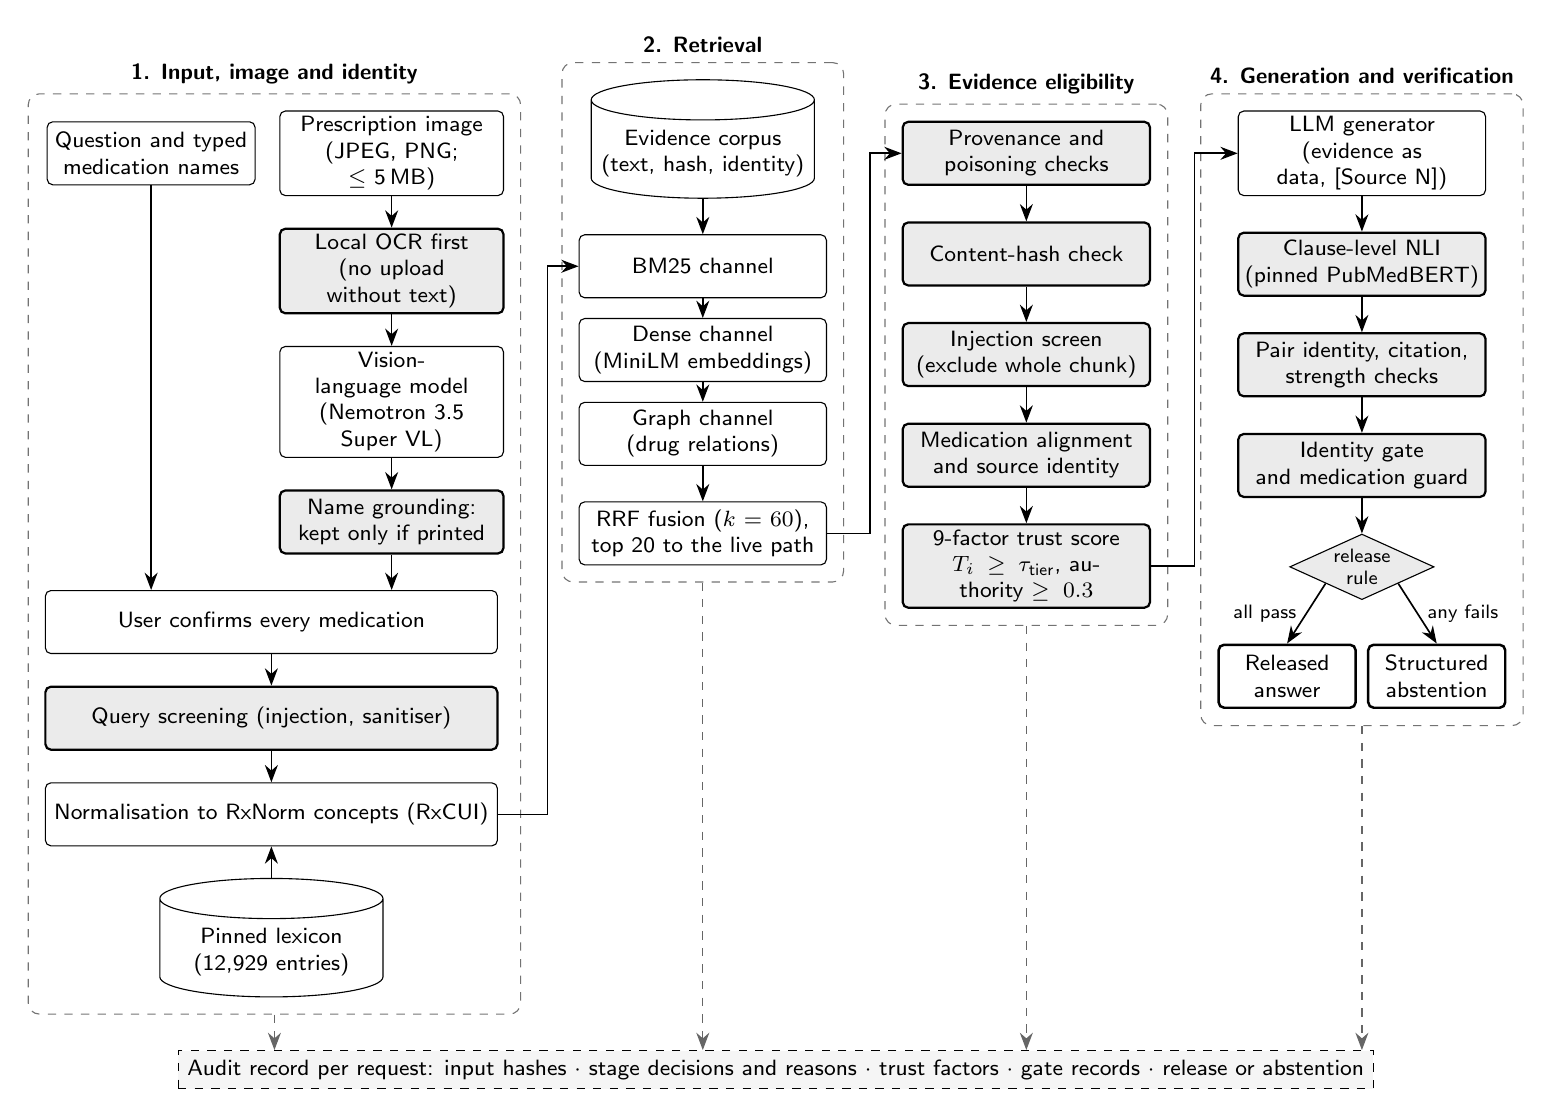
\begin{tikzpicture}[
  font=\sffamily\footnotesize, >={Stealth[length=2.2mm]},
  box/.style={draw, rounded corners=2pt, fill=white, align=center, text width=3.0cm, minimum height=0.8cm, inner sep=2pt},
  ctl/.style={box, fill=black!8, line width=0.8pt},
  store/.style={draw, cylinder, shape border rotate=90, aspect=0.18, fill=white, align=center, text width=2.6cm, minimum height=0.95cm},
  dec/.style={draw, diamond, aspect=2.2, fill=black!8, align=center, inner sep=0.5pt, font=\sffamily\scriptsize},
  outbox/.style={box, text width=1.6cm, line width=0.9pt},
  stage/.style={draw=black!55, dashed, rounded corners=4pt, inner sep=6pt},
  slabel/.style={font=\sffamily\bfseries\footnotesize, anchor=south},
  flow/.style={->, line width=0.6pt}, logl/.style={->, dashed, black!60, line width=0.5pt}]
% stage 1: input, image path and identity
\node[box, text width=2.5cm] (q) {Question and typed\\medication names};
\node[box, right=0.3cm of q, text width=2.7cm] (img) {Prescription image\\(JPEG, PNG; $\le$ 5\,MB)};
\node[ctl, below=0.4cm of img, text width=2.7cm] (ocr) {Local OCR first\\(no upload without text)};
\node[box, below=0.4cm of ocr, text width=2.7cm] (vlm) {Vision-language model\\(Nemotron 3.5 Super VL)};
\node[ctl, below=0.4cm of vlm, text width=2.7cm] (gnd) {Name grounding:\\kept only if printed};
\path (q.center) -- (img.center) coordinate[pos=0.5] (mid);
\node[box, text width=5.6cm, anchor=north] (conf) at ([yshift=-0.45cm]gnd.south -| mid) {User confirms every medication};
\node[ctl, below=0.4cm of conf, text width=5.6cm] (sec) {Query screening (injection, sanitiser)};
\node[box, below=0.4cm of sec, text width=5.6cm] (norm) {Normalisation to RxNorm concepts (RxCUI)};
\node[store, below=0.4cm of norm] (lex) {Pinned lexicon\\(12{,}929 entries)};
% stage 2: retrieval
\node[store, right=1.1cm of img] (corp) {Evidence corpus\\(text, hash, identity)};
\node[box, below=0.45cm of corp] (bm) {BM25 channel};
\node[box, below=0.25cm of bm] (dn) {Dense channel\\(MiniLM embeddings)};
\node[box, below=0.25cm of dn] (gr) {Graph channel\\(drug relations)};
\node[box, below=0.45cm of gr] (rrf) {RRF fusion ($k=60$),\\top 20 to the live path};
% stage 3: evidence eligibility
\node[ctl, right=1.1cm of corp] (pois) {Provenance and\\poisoning checks};
\node[ctl, below=0.45cm of pois] (hash) {Content-hash check};
\node[ctl, below=0.45cm of hash] (inj) {Injection screen\\(exclude whole chunk)};
\node[ctl, below=0.45cm of inj] (align) {Medication alignment\\and source identity};
\node[ctl, below=0.45cm of align] (tr) {9-factor trust score\\$T_i\ge\tau_{\text{tier}}$, authority $\ge 0.3$};
% stage 4: generation and verification
\node[box, right=1.1cm of pois] (gen) {LLM generator\\(evidence as data, [Source N])};
\node[ctl, below=0.45cm of gen] (nli) {Clause-level NLI\\(pinned PubMedBERT)};
\node[ctl, below=0.45cm of nli] (cid) {Pair identity, citation,\\strength checks};
\node[ctl, below=0.45cm of cid] (gate) {Identity gate\\and medication guard};
\node[dec, below=0.45cm of gate] (d) {release\\rule};
\node[outbox, below=0.55cm of d, xshift=-0.95cm] (ans) {Released\\answer};
\node[outbox, below=0.55cm of d, xshift=0.95cm] (abs) {Structured\\abstention};
\begin{scope}[on background layer]
\node[stage, fit=(q)(img)(lex)(conf)] (S1) {}; \node[stage, fit=(corp)(rrf)] (S2) {};
\node[stage, fit=(pois)(tr)] (S3) {}; \node[stage, fit=(gen)(ans)(abs)] (S4) {};
\end{scope}
\node[slabel] at (S1.north) {1. Input, image and identity}; \node[slabel] at (S2.north) {2. Retrieval};
\node[slabel] at (S3.north) {3. Evidence eligibility}; \node[slabel] at (S4.north) {4. Generation and verification};
\draw[flow] (img)--(ocr); \draw[flow] (ocr)--(vlm); \draw[flow] (vlm)--(gnd);
\draw[flow] (gnd.south) -- (gnd.south |- conf.north);
\draw[flow] (q.south) -- (q.south |- conf.north);
\draw[flow] (conf)--(sec); \draw[flow] (sec)--(norm); \draw[flow] (lex)--(norm);
\draw[flow] (corp)--(bm); \draw[flow] (bm)--(dn); \draw[flow] (dn)--(gr); \draw[flow] (gr)--(rrf);
\draw[flow] (norm.east) -- ($(norm.east -| corp.west)+(-0.55,0)$) |- (bm.west);
\draw[flow] (rrf.east) -- ++(0.55,0) |- (pois.west);
\draw[flow] (pois)--(hash); \draw[flow] (hash)--(inj); \draw[flow] (inj)--(align); \draw[flow] (align)--(tr);
\draw[flow] (tr.east) -- ++(0.55,0) |- (gen.west);
\draw[flow] (gen)--(nli); \draw[flow] (nli)--(cid); \draw[flow] (cid)--(gate); \draw[flow] (gate)--(d);
\draw[flow] (d.south west) -- node[left,font=\sffamily\scriptsize]{all pass} (ans.north);
\draw[flow] (d.south east) -- node[right,font=\sffamily\scriptsize]{any fails} (abs.north);
\coordinate (midx) at ($(S1.south west)!0.5!(S4.south east)$);
\node[draw, dashed, fill=black!4, align=center, font=\sffamily\footnotesize, anchor=north] (log)
  at ([yshift=-0.45cm]midx |- S1.south)
  {Audit record per request: input hashes $\cdot$ stage decisions and reasons $\cdot$ trust factors $\cdot$ gate records $\cdot$ release or abstention};
\draw[logl] (S1.south) -- (S1.south |- log.north); \draw[logl] (S2.south) -- (S2.south |- log.north);
\draw[logl] (S3.south) -- (S3.south |- log.north); \draw[logl] (S4.south) -- (S4.south |- log.north);
\end{tikzpicture}}
\caption{Architecture of the final candidate (C2j). Shaded nodes are the controls added to a conventional RAG pipeline.
An uploaded image is read by local OCR before anything leaves the machine; the vision model's names are kept only if
they are printed on the image, and the user confirms every medication. A failed exclusion check removes a chunk; a
failed claim check withholds the whole answer.}
\label{fig:arch}
\end{figure*}

\subsection{Input, identity and retrieval}

Medication names are extracted from the request, confirmed by the user and resolved against a pinned RxNorm
prescribable lexicon \cite{nelson2011rxnorm} (12{,}929 entries) and a curated RxCUI cache; brands, ingredients and salts
remain distinct concepts. A prescription image is first read by local OCR; it is sent to the vision-language model
only if that OCR finds text, and a returned name is offered for confirmation only if it is printed on the image.
Retrieval runs three channels over the same corpus: BM25 over lower-cased tokens
\cite{robertson2009bm25}, cosine similarity over \texttt{all-MiniLM-L6-v2} embeddings \cite{reimers2019sbert}, and an
adjacency-list graph of drug relations seeded with the confirmed medications. Reciprocal rank fusion
\begin{equation}
\mathrm{RRF}(d) = \sum_{r \in \mathcal{L}} \frac{1}{k + \mathrm{rank}_r(d)}, \qquad k = 60,
\label{eq:rrf}
\end{equation}
merges the lists \cite{cormack2009rrf}; at most 50 fused candidates are kept, chunks with a poisoning score above 0.4
are dropped, and the live path requests the top 20.

\subsection{Evidence eligibility and trust}

Each candidate $e_i$ passes five exclusion checks: a provenance poisoning check; equality of the SHA-256 of its text with
the registered content hash; an injection screen that excludes the whole chunk (stripping the instruction would change
the hashed evidence); medication alignment (the chunk must name a requested medication); and verified source identity.
Duplicate texts are kept once. Surviving chunks receive a trust score over nine factors $f_{ik} \in [0,1]$,
\begin{equation}
T_i = \sum_{k=1}^{9} w_{k}^{(r)} f_{ik}, \qquad \sum_k w_k^{(r)} = 1,
\label{eq:trust}
\end{equation}
whose weights $w^{(r)}$ depend on the risk tier $r \in \{\mathrm{R0},\dots,\mathrm{R3}\}$ of the question
(Table~\ref{tab:trust}). A factor that the evidence record does not carry is treated as missing and contributes zero, so
a gap never raises the score. The eligibility decision is
\begin{equation}
G_i = \big[\,\text{passes all exclusions}\,\big] \wedge \big[\,T_i \ge \tau_r\,\big] \wedge \big[\,A_i \ge 0.3\,\big],
\label{eq:gate}
\end{equation}
with $\tau = (0.30, 0.45, 0.60, 0.75)$ for R0 to R3 and $A_i$ the source authority. Adversarial risk enters as hard
exclusions and as the anti-poisoning and anti-injection factors, so a high trust score cannot buy back a security flag.
The trust score filters chunks; it does not reorder them, so eligible evidence keeps its fused rank.

\begin{table}[!t]
\caption{Trust factor weights per risk tier (configuration of C2h)}
\label{tab:trust}
\centering
\footnotesize
\begin{tabular}{@{}lcccc@{}}
\toprule
Factor & R0 & R1 & R2 & R3 \\
\midrule
Source authority & 0.15 & 0.20 & 0.25 & 0.30 \\
Query relevance & 0.20 & 0.20 & 0.15 & 0.10 \\
Evidence quality & 0.10 & 0.15 & 0.20 & 0.25 \\
Freshness & 0.10 & 0.10 & 0.10 & 0.10 \\
Consistency & 0.15 & 0.10 & 0.10 & 0.10 \\
Entity match & 0.10 & 0.10 & 0.10 & 0.10 \\
Population match & 0.05 & 0.05 & 0.05 & 0.03 \\
Anti-poisoning & 0.10 & 0.05 & 0.03 & 0.01 \\
Anti-injection & 0.05 & 0.05 & 0.02 & 0.01 \\
\midrule
Threshold $\tau_r$ & 0.30 & 0.45 & 0.60 & 0.75 \\
\bottomrule
\end{tabular}
\end{table}

\subsection{Claim verification and release}

Eligible chunks are numbered and passed to the generator as data, and each claim must cite them with \texttt{[Source N]}
markers. Each generated claim $c$ is then checked four ways. A pinned NLI model (PubMedBERT fine-tuned on MNLI and MedNLI,
at a fixed revision \cite{gu2021pubmedbert,romanov2018mednli}) judges each clause against its cited chunk, so one
unsupported clause makes the claim unsupported; an aggregate check considers all retrieved chunks. A pair-identity
check compares the drug pair, relation and direction with an approved relationship record. Citation checks resolve each
marker to an eligible chunk and check alignment and claim strength. The medication identity gate requires every
medication or class that the claim puts in a drug role to be named word for word by a cited source (text or verified
title), resolving anaphors and rejecting unresolved or invented names; a separate guard rejects medications the user did
not confirm. The release predicate is
\begin{equation}
\begin{split}
\mathrm{Release}(c) = {}& [\,s(c) = \textsc{supported}\,] \wedge [\,g(c) = \textsc{pass}\,]\\
& \wedge [\,m(c) = \varnothing\,],
\end{split}
\label{eq:release}
\end{equation}
where $s$ is the final support state, $g$ the gate decision and $m$ the guard message. The predicate reads the gate and
guard records directly, so no later stage can restore a rejected claim, and a claim without a gate record fails.
Withheld claims produce a structured abstention with the stage and reason.




%% =====================================================================================================================
\section{Algorithms}
\label{sec:algo}

Algorithms~\ref{alg:admit} and~\ref{alg:verify} give the two stages as implemented. Admission applies every
exclusion before the trust score, so a chunk that fails one is never scored, and an empty evidence pack ends the
request with an abstention before any model is called. Verification runs the verifier and the identity gate on every
claim, and the strength, citation-alignment and guard checks on every claim the verifier passes, and records each
result even when an earlier check has already failed; release requires all of them~\eqref{eq:release}. Because the
results are recorded separately, the release decision under any subset of the checks can be recomputed from stored
runs (Section~\ref{sec:contrib}).

\begin{algorithm}[!t]
\caption{Evidence admission (pre-generation)}
\label{alg:admit}
\begin{algorithmic}[1]
\Require query $Q$, confirmed medications $D$; tier thresholds $\tau$
\Ensure numbered evidence pack $\mathcal{P}$ or abstention
\State screen and sanitise $Q$; resolve $D$ in the pinned lexicon
\State $\mathcal{E} \gets$ RRF of BM25, dense and graph rankings \eqref{eq:rrf}; drop poisoning score $> 0.4$
\State $r \gets$ risk tier of $Q$; $\mathcal{P} \gets \emptyset$
\For{each $e_i \in \mathcal{E}$ in fused order}
  \If{provenance blocked \textbf{or} hash mismatch \textbf{or} carries instructions} \textbf{continue} \EndIf
  \If{$e_i$ names no medication in $D$ \textbf{or} identity unverified} \textbf{continue} \EndIf
  \If{text already in $\mathcal{P}$} \textbf{continue} \EndIf
  \State $T_i \gets$ \eqref{eq:trust} with missing factors set to 0
  \If{$T_i \ge \tau_r$ \textbf{and} $A_i \ge 0.3$} $\mathcal{P} \gets \mathcal{P} \cup \{e_i\}$ \EndIf
\EndFor
\If{$\mathcal{P} = \emptyset$} \Return abstention (no eligible evidence) \EndIf
\State \Return $\mathcal{P}$ numbered as [Source 1..N]
\end{algorithmic}
\end{algorithm}

\begin{algorithm}[!t]
\caption{Claim verification and release (post-generation)}
\label{alg:verify}
\begin{algorithmic}[1]
\Require answer $y$ generated from $\mathcal{P}$; confirmed medications $D$
\Ensure released claims and abstentions with reasons
\For{each claim $c$ in $y$}
  \State $s(c) \gets$ clause-level NLI on cited chunks, aggregate check, pair identity, citation and strength checks
  \State $g(c) \gets$ identity gate on drug-role names vs.\ cited text and titles
  \State $m(c) \gets$ guard: medications named but not in $D$
  \If{\eqref{eq:release} holds} release $c$ \Else\ withhold $c$ and record the first failing stage \EndIf
\EndFor
\end{algorithmic}
\end{algorithm}

%% =====================================================================================================================
\section{Data and Evidence Management}
\label{sec:data}

Every chunk carries a provenance record: source type, document identifier, URL, retrieval time, content hash and, where
established, a source-identity record with title and version. The evaluated local corpus has 17 items. All 17 content
hashes match their text, but only the three DailyMed label sections (lisinopril sections 5.5 and 7.1, warfarin sodium
section 7.3) have a verified source identity; the other 14 chunks have none and 11 carry placeholder URLs, and no
relationship record has owner approval. A matching hash shows that stored text is unchanged; it does not show that the
text came from the claimed source. DailyMed shows each product's in-use labeling, which may differ from the latest
FDA-approved labeling, so set identifier, version, section and retrieval date are kept with each item.

%% =====================================================================================================================
\section{Evaluation Method}
\label{sec:method}

Apart from the pilot in Section~\ref{sec:live}, all runs used an isolated copy of the frozen candidate, offline, with
the pinned NLI model and no provider call.
Generation was scripted: each test statement is fed through the real release path as if a model had written it, so the
checks are measured, not a language model. A statement can stop in four places: before the identity gate (no
eligible evidence), at the gate, after it, or released; counting an upstream abstention as a gate rejection would
credit the gate for work it did not do, so we report each separately. Seven constructed statement sets (V2 to V8,
731 scored rows; row counts in Table~\ref{tab:gate}) were written
during development, each after the previous candidate had been tested, so they are development-informed regression
sets; V8 was written by the author of C2h and is author-known. Each row is labelled PASS (every medication or class in a
drug role is named by the cited source) or REJECT, with the expected failing entity. All labels are AI-written and
unreviewed; blind review packets with opaque identifiers are prepared.


For each set we report the gate miss rate (REJECT rows the gate passed, over REJECT rows that reached it), unsupported
releases (REJECT rows released), the identity false-withhold rate (PASS rows the gate rejected, over PASS rows) and
coverage (PASS rows released). Rates carry 95\% intervals: Clopper and Pearson's exact interval \cite{clopper1934}
when the count is 0 and Wilson's interval \cite{wilson1927} otherwise. Paired comparisons on the same rows use the
exact McNemar test \cite{mcnemar1947}. Sets are never pooled into one rate. The acceptance criterion for identity false
withholds, fixed before any new confirmation set, is a point estimate of at most 5\% with the Wilson interval reported.

%% =====================================================================================================================
\section{Results}
\label{sec:results}

\begin{figure*}[!t]
\centering
\resizebox{\textwidth}{!}{%
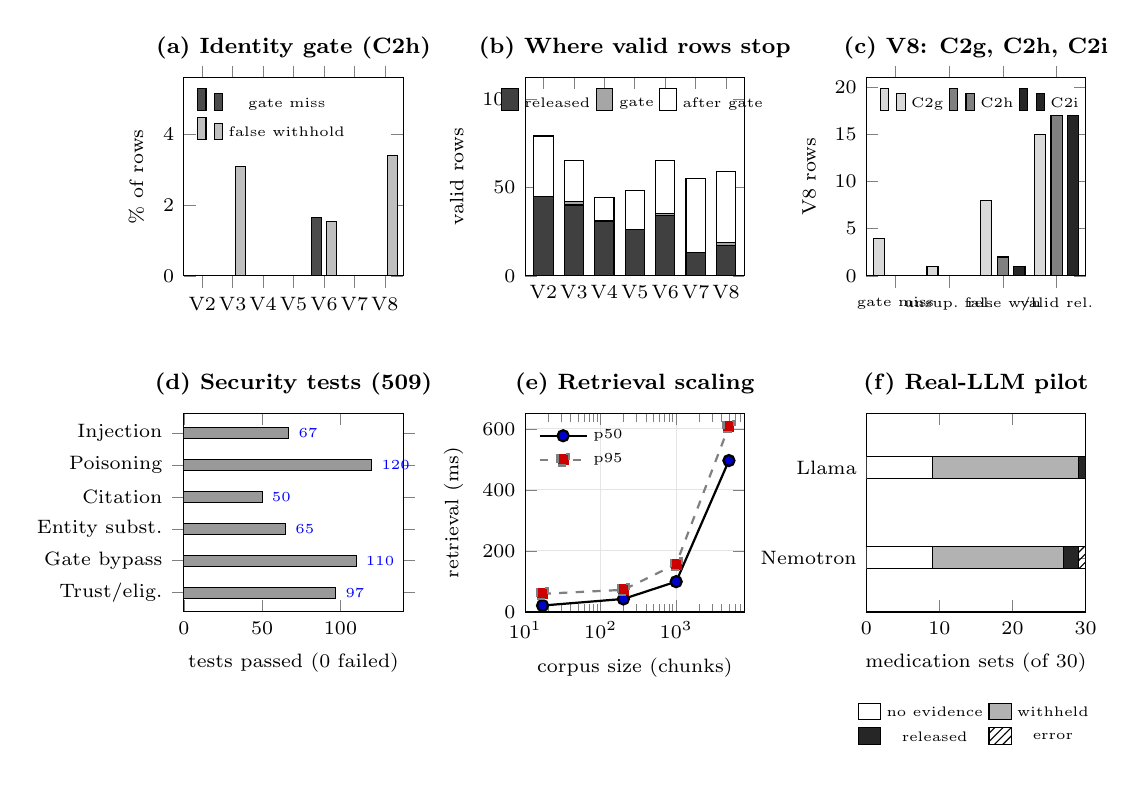
\begin{tikzpicture}
\begin{groupplot}[group style={group size=3 by 2, horizontal sep=1.55cm, vertical sep=1.75cm},
  width=0.36\textwidth, height=4.1cm, tick label style={font=\scriptsize}, label style={font=\scriptsize},
  title style={font=\footnotesize\bfseries, yshift=-1mm}, legend style={font=\tiny, draw=none, fill=none}]
% (a) gate misses and identity false withholds
\nextgroupplot[ybar, bar width=3.5pt, ymin=0, ymax=5.6, ylabel={\% of rows}, title={(a) Identity gate (C2h)},
  symbolic x coords={V2,V3,V4,V5,V6,V7,V8}, xtick=data, enlarge x limits=0.1,
  legend style={at={(0.02,0.98)}, anchor=north west}]
\addplot+[fill=black!70, draw=black] coordinates {(V2,0) (V3,0) (V4,0) (V5,0) (V6,1.64) (V7,0) (V8,0)};
\addplot+[fill=black!25, draw=black] coordinates {(V2,0) (V3,3.08) (V4,0) (V5,0) (V6,1.54) (V7,0) (V8,3.39)};
\legend{gate miss, false withhold}
% (b) stop points of valid statements
\nextgroupplot[ybar stacked, bar width=7pt, ymin=0, ymax=112, ylabel={valid rows}, title={(b) Where valid rows stop},
  symbolic x coords={V2,V3,V4,V5,V6,V7,V8}, xtick=data, enlarge x limits=0.1, legend columns=3,
  legend style={at={(0.5,0.98)}, anchor=north}]
\addplot+[fill=black!75, draw=black] coordinates {(V2,45) (V3,40) (V4,31) (V5,26) (V6,34) (V7,13) (V8,17)};
\addplot+[fill=black!35, draw=black] coordinates {(V2,0) (V3,2) (V4,0) (V5,0) (V6,1) (V7,0) (V8,2)};
\addplot+[fill=white, draw=black] coordinates {(V2,34) (V3,23) (V4,13) (V5,22) (V6,30) (V7,42) (V8,40)};
\legend{released, gate, after gate}
% (c) three code versions on V8
\nextgroupplot[ybar, bar width=4pt, ymin=0, ymax=21, ylabel={V8 rows}, title={(c) V8: C2g, C2h, C2i},
  symbolic x coords={miss,rel,fw,cov}, xtick=data, xticklabels={gate miss, unsup. rel., false w/h, valid rel.},
  x tick label style={font=\tiny}, enlarge x limits=0.18, legend columns=3, legend style={at={(0.02,0.98)}, anchor=north west}]
\addplot+[fill=black!15, draw=black] coordinates {(miss,4) (rel,1) (fw,8) (cov,15)};
\addplot+[fill=black!50, draw=black] coordinates {(miss,0) (rel,0) (fw,2) (cov,17)};
\addplot+[fill=black!85, draw=black] coordinates {(miss,0) (rel,0) (fw,1) (cov,17)};
\legend{C2g, C2h, C2i}
% (d) security tests by group
\nextgroupplot[xbar, bar width=4pt, xmin=0, xmax=140, xlabel={tests passed (0 failed)}, title={(d) Security tests (509)},
  symbolic y coords={Trust/elig.,Gate bypass,Entity subst.,Citation,Poisoning,Injection}, ytick=data,
  nodes near coords, nodes near coords style={font=\tiny}, enlarge y limits=0.12]
\addplot+[fill=black!40, draw=black] coordinates {(97,Trust/elig.) (110,Gate bypass) (65,Entity subst.) (50,Citation) (120,Poisoning) (67,Injection)};
% (e) retrieval scaling
\nextgroupplot[xmode=log, xmin=10, xmax=8000, ymin=0, ymax=650, xlabel={corpus size (chunks)},
  ylabel={retrieval (ms)}, title={(e) Retrieval scaling}, grid=major, grid style={black!10},
  legend style={at={(0.02,0.98)}, anchor=north west}]
\addplot+[mark=*, black, thick] coordinates {(17,21.046) (200,42.606) (1000,99.303) (5000,496.249)};
\addplot+[mark=square*, black!50, thick, dashed] coordinates {(17,59.449) (200,72.521) (1000,156.842) (5000,608.75)};
\legend{p50, p95}
% (f) real-LLM pilot outcomes
\nextgroupplot[xbar stacked, bar width=8pt, xmin=0, xmax=30, xlabel={medication sets (of 30)},
  title={(f) Real-LLM pilot}, symbolic y coords={Nemotron,Llama}, ytick=data, enlarge y limits=0.6,
  legend columns=2, legend style={at={(0.5,-0.42)}, anchor=north}]
\addplot+[fill=white, draw=black] coordinates {(9,Llama) (9,Nemotron)};
\addplot+[fill=black!30, draw=black] coordinates {(20,Llama) (18,Nemotron)};
\addplot+[fill=black!85, draw=black] coordinates {(1,Llama) (2,Nemotron)};
\addplot+[pattern=north east lines, draw=black] coordinates {(0,Llama) (1,Nemotron)};
\legend{no evidence, withheld, released, error}
\end{groupplot}
\end{tikzpicture}}
\caption{Results at a glance. (a) Gate misses and identity false withholds per development set (C2h; exact intervals
in Table~\ref{tab:gate}). (b) Where valid statements stop (\texttt{OFFLINE\_METRICS\_01}). (c) Three code versions on
the same V8 statements (\texttt{V8\_PAIRED\_C2G\_C2H\_01}, \texttt{C2H\_VS\_C2I\_02}; V8 is author-known). (d) Scoped
security tests by threat group, all passing on C2h, C2i and C2j. (e) Hybrid retrieval latency on synthetic corpora
(\texttt{PF01\_SCALING\_01}). (f) Terminal outcome per medication set in the real-LLM pilot (\texttt{LIVE\_TEXT\_01},
\texttt{\_03}).}
\label{fig:results}
\end{figure*}

\subsection{Reproducibility}

A clean offline rerun of the frozen candidate produced 15 of 15 result files byte-identical to the stored reference, and
the backend suite gave 2{,}252 passed, 0 failed and 4 skipped (provider credentials absent) in normal and
network-blocked modes (run \texttt{C2H\_REPRO\_01}).

\subsection{Identity gate}

Table~\ref{tab:gate} and Fig.~\ref{fig:results}a give the per-set results. No REJECT row was released in any set. Among REJECT
rows that reached the gate, the gate passed one (V6-IND-03, a row whose label is a recorded error). One REJECT row
(V7-SRC-02) never reached the gate: its cited section names neither requested medication, so the pipeline abstained
before generation. On V8 the two false withholds came from the ordinary words ``nudge'' and ``oozing'', which the gate's
word list did not contain (Fig.~\ref{fig:compare}b).

\begin{table}[!t]
\caption{Identity gate per development set (C2h; runs \texttt{STOP\_POINTS\_SUPPLEMENTARY\_01}, \texttt{OFFLINE\_METRICS\_01})}
\label{tab:gate}
\centering
\footnotesize
\setlength{\tabcolsep}{3pt}
\begin{tabular}{@{}lcccc@{}}
\toprule
Set & Gate miss & Not & False withhold & Coverage \\
 & (95\% CI, \%) & reached & (95\% CI, \%) & \\
\midrule
V2 & 0/40 (0, 8.8) & 0 & 0/79 (0, 4.6) & 45/79 \\
V3 & 0/36 (0, 9.7) & 0 & 2/65 (0.9, 10.5) & 40/65 \\
V4 & 0/28 (0, 12.3) & 0 & 0/44 (0, 8.0) & 31/44 \\
V5 & 0/36 (0, 9.7) & 0 & 0/48 (0, 7.4) & 26/48 \\
V6 & 1/61 (0.3, 8.7) & 0 & 1/65 (0.3, 8.2) & 34/65 \\
V7 & 0/60 (0, 6.0) & 1 & 0/55 (0, 6.5) & 13/55 \\
V8 & 0/54 (0, 6.6) & 0 & 2/59 (0.9, 11.5) & 17/59 \\
\bottomrule
\multicolumn{5}{@{}l}{\scriptsize Unsupported releases: 0 in every set. Labels AI-written; sets development-informed.}
\end{tabular}
\end{table}


\subsection{Where valid statements stop}

Coverage is low (Fig.~\ref{fig:results}b). Across V2 to V8, 206 valid statements were released, 5 were rejected by the
identity gate and 204 passed the gate and were withheld later (run \texttt{STOP\_DIAGNOSTICS\_C2H\_01}). The first
stage to withhold them was NLI in 129 (entailment below 0.10 in 101), pair identity in 52, the verifier's aggregate
check in 18 and the medication guard in 5. The pair-identity stops follow from
missing or unapproved relationship records (34 claims whose canonical identity was not resolved, 18 whose source identity
was unavailable), so they are correct under the current evidence. Whether the NLI and aggregate stops are right cannot
be decided without claim-support labels. The five guard stops are a defect: the guard reported the ordinary words
``Perform'' (three times), ``Align'' and ``sodium'' as unconfirmed medications although the gate had passed them.
``Perform'' and ``Align'' are RxNorm brand names opening an instruction (``Perform potassium monitoring
periodically''), and ``sodium'' occurs in ``a low-sodium diet''.



\subsection{What each check contributes}
\label{sec:contrib}

Because every check result is recorded, we recomputed the release decision of every
development row under subsets of the checks (Table~\ref{tab:contrib} and Fig.~\ref{fig:compare}a; run \texttt{CHECK\_COUNTERFACTUAL\_01}).
Recomputing the full rule reproduced the recorded outcome on all 731 rows. A conventional pipeline~\eqref{eq:baseline}
fed the same scripted statements shows all of them, including every REJECT row. With every check except the
identity gate, 3 to 19 identity-unsupported statements per set would have been released (75 rows in the seven sets).
In these rows the NLI model found the claim entailed by its cited chunk, but the chunk does not name a medication or
class that the claim asserts: invented names (``Duskwell can raise the bleeding hazard for warfarin users'') and
classes that the warfarin or lisinopril section does not name (``SSRIs may call for closer INR follow-up in warfarin
users''). The identity gate alone released one REJECT row (V6-IND-03, the recorded label error) and withheld no valid
row apart from its own false withholds, but it checks no semantic support; the full rule released 13 to 45 valid rows
per set. The sets were written to exercise the gate, so these counts show what the other checks miss on such
statements, not how often such statements occur in real answers.

\begin{table}[!t]
\caption{Rows released under subsets of the checks, recomputed from recorded results (C2h; run
\texttt{CHECK\_COUNTERFACTUAL\_01})}
\label{tab:contrib}
\centering
\footnotesize
\setlength{\tabcolsep}{3pt}
\begin{tabular}{@{}lrrrr@{\hspace{10pt}}rrr@{}}
\toprule
 & \multicolumn{4}{c}{REJECT rows released} & \multicolumn{3}{c}{PASS rows released} \\
\cmidrule(lr){2-5}\cmidrule(l){6-8}
Set & none & gate only & all but gate & all & of & gate only & all \\
\midrule
V2 & 40/40 & 0 & 14 & 0 & 79 & 79 & 45 \\
V3 & 36/36 & 0 & 14 & 0 & 65 & 63 & 40 \\
V4 & 28/28 & 0 & 5 & 0 & 44 & 44 & 31 \\
V5 & 36/36 & 0 & 3 & 0 & 48 & 48 & 26 \\
V6 & 61/61 & 1 & 19 & 0 & 65 & 64 & 34 \\
V7 & 61/61 & 0 & 10 & 0 & 55 & 55 & 13 \\
V8 & 54/54 & 0 & 10 & 0 & 59 & 57 & 17 \\
\bottomrule
\multicolumn{8}{@{}L{0.95\columnwidth}@{}}{\scriptsize ``None'': no eligibility stage and no check, as in
\eqref{eq:baseline}; the other columns keep the eligibility stage, which stopped V7-SRC-02. Scripted generation;
labels AI-written; sets development-informed.}
\end{tabular}
\end{table}

\begin{figure}[!t]
\centering
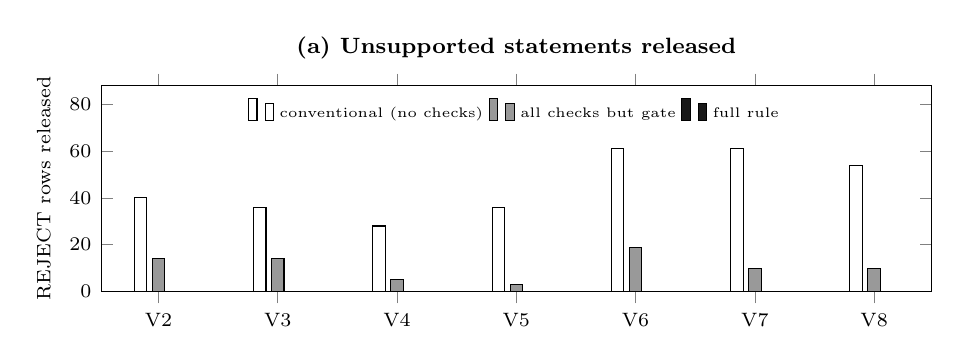
\begin{tikzpicture}
\begin{axis}[ybar, width=\columnwidth, height=4.2cm, bar width=4.5pt, ymin=0, ymax=88,
  ylabel={REJECT rows released}, ylabel style={font=\scriptsize}, tick label style={font=\scriptsize},
  symbolic x coords={V2,V3,V4,V5,V6,V7,V8}, xtick=data, enlarge x limits=0.08,
  legend style={font=\tiny, at={(0.5,0.97)}, anchor=north, legend columns=3, draw=none},
  title={(a) Unsupported statements released}, title style={font=\footnotesize\bfseries}]
\addplot+[fill=white, draw=black] coordinates {(V2,40) (V3,36) (V4,28) (V5,36) (V6,61) (V7,61) (V8,54)};
\addplot+[fill=black!40, draw=black] coordinates {(V2,14) (V3,14) (V4,5) (V5,3) (V6,19) (V7,10) (V8,10)};
\addplot+[fill=black!90, draw=black] coordinates {(V2,0) (V3,0) (V4,0) (V5,0) (V6,0) (V7,0) (V8,0)};
\legend{conventional (no checks), all checks but gate, full rule}
\end{axis}
\end{tikzpicture}

\vspace{2mm}
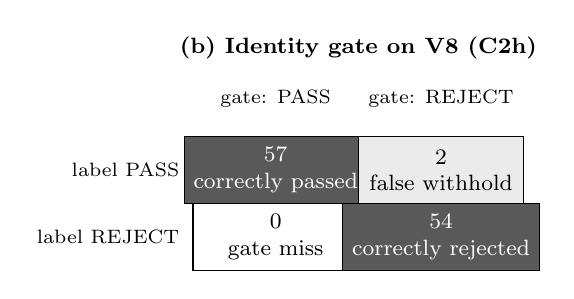
\begin{tikzpicture}[cell/.style={draw, minimum width=2.1cm, minimum height=0.85cm, align=center, font=\footnotesize},
  hd/.style={font=\scriptsize, align=center}]
\node[font=\footnotesize\bfseries] at (2.1,1.55) {(b) Identity gate on V8 (C2h)};
\node[hd] at (1.05,0.9) {gate: PASS}; \node[hd] at (3.15,0.9) {gate: REJECT};
\node[hd, anchor=east] at (-0.05,0) {label PASS}; \node[hd, anchor=east] at (-0.05,-0.85) {label REJECT};
\node[cell, fill=black!65, text=white] at (1.05,0) {57\\correctly passed};
\node[cell, fill=black!8] at (3.15,0) {2\\false withhold};
\node[cell, fill=black!0] at (1.05,-0.85) {0\\gate miss};
\node[cell, fill=black!65, text=white] at (3.15,-0.85) {54\\correctly rejected};
\end{tikzpicture}
\caption{(a) Unsupported (REJECT) statements released per development set by a conventional pipeline, by every check
except the identity gate, and by the full release rule, recomputed from recorded results (C2h;
\texttt{CHECK\_COUNTERFACTUAL\_01}; Table~\ref{tab:contrib}). (b) Confusion matrix of the identity gate on the 113 V8
statements (Table~\ref{tab:gate}); the two false withholds are the words ``nudge'' and ``oozing''. Labels are
AI-written and V8 is author-known.}
\label{fig:compare}
\end{figure}

\subsection{Candidate comparison and remediation}

On the same 113 V8 statements (Fig.~\ref{fig:results}c), the previous candidate's code (C2g) had 4 gate misses, 1 unsupported release, 8 false
withholds and 15 valid releases; C2h had 0, 0, 2 and 17. C2h fixed 10 decisions and broke none (exact McNemar
$p=0.002$; runs \texttt{V8\_PAIRED\_C2G\_C2H\_01}, \texttt{V8\_RISK\_COVERAGE\_01}); since V8 is author-known,
this is exploratory.

We then built a remediation candidate (C2i) from C2h to fix the two defects found above without loosening any check.
First, an ordinary verb is now known when its listed past or present participle is (the word list held ``nudged'' but
not ``nudge''); plural forms are not used, so a name whose plural happens to be listed is not made known. Second, the
guard skips an unconfirmed finding only in two forms: an RxNorm brand name that is an ordinary English word, opens a
sentence and is not followed by a modal or auxiliary (``Perform potassium monitoring'', but not ``Perform may raise
\dots''), and an ingredient inside a ``low-'', ``high-'' or ``reduced-'' diet compound. A brand used anywhere else, a
brand that is not an ordinary word (``Advil''), an everyday-word ingredient such as lithium, and every confirmed or
unresolved name are still reported; 52 new unit tests pin these cases. Across all 731 development rows six decisions
changed, none for the worse (run \texttt{C2H\_VS\_C2I\_02}): the five guard rows (H-CWD-04, H-CWD-08, V3-CWD-03,
V5-CW-04, V6-NPH-04) are now released, and the ``nudge'' statement (V8-SRC-08) passes the gate but is still withheld
by pair identity. No unsupported statement
was released, the 42-example NLI replay was unchanged, the 509 security tests passed and the backend suite gave
2{,}304 passed, 0 failed and 4 skipped with the network blocked (run \texttt{C2I\_REGRESSION\_02}). ``Oozing'' remains unfixed because no vocabulary we could audit offline contains any form of ``ooze''.
V2 to V8 informed these changes, so these are development-set results.



\subsection{Security regression}

We grouped 509 existing tests by threat and ran them with the network blocked (Fig.~\ref{fig:results}d): prompt injection 67, poisoning and
provenance 120, citation manipulation 50, entity substitution 65, gate bypass and fallback 110, trust and
eligibility 97. All passed on C2h, on C2i and on C2j (runs \texttt{SECURITY\_REGRESSION\_01},
\texttt{C2J\_PORT\_CANCELLATION\_01}). The tests check specified behaviours with inputs written by the developers; they are not an attack-success rate,
and a 110-case security set stays unrun until people review its labels.


\subsection{Performance}

On one CPU machine with a warm file cache and the 17-item corpus, median latency was 7.9~ms for retrieval
($n=63$), 1.4~ms for the identity gate per statement ($n=635$) and 164.6~ms for the full offline release path
($n=339$; 95th percentile 336.7~ms); peak working set was 837~MB (run \texttt{PF01\_OFFLINE\_LATENCY\_02}). These
figures exclude any language-model call. On C2j (\texttt{PF01\_C2J\_SUPPLEMENT\_01}) one NLI pair took 254.9~ms
(median; p95 478.9~ms), local OCR 1.05~s per image, grounding under 2~ms and name normalisation 0.03~ms.

To see how retrieval scales, we built the unmodified hybrid retriever over synthetic, fictional corpora of 17, 200,
1{,}000 and 5{,}000 chunks and timed the same 30 queries after 5 warm-up queries (run \texttt{PF01\_SCALING\_01}; Fig.~\ref{fig:results}e). Median latency grew from 21.0~ms to 42.6, 99.3 and 496.2~ms, roughly linearly with corpus
size, because the dense channel scores every chunk by brute-force cosine similarity; building the index (tokenising and
embedding) took 1.2~s, 7.7~s, 39.1~s and 183.7~s, and peak working set reached 980~MB at 5{,}000 chunks. This harness
encodes each query with the sentence-transformer directly, so its 17-chunk figure is not comparable with the 7.9~ms
above. A production corpus would need an approximate nearest-neighbour index; the synthetic text says nothing about
retrieval quality.


\subsection{Pilot with real language models}
\label{sec:live}

Everything above used scripted generation. To see how the release path handles text a model actually writes, we ran a
small authorised pilot on C2i with two hosted models, Llama~3.3 70B Instruct on Cloudflare Workers AI and Nemotron~3
Ultra on NVIDIA's API. Each received the same 30 synthetic medication sets once: 15 with warfarin, 5 with lisinopril
and 10 control sets with no evidence in the corpus. Only synthetic inputs and the three public DailyMed sections were
sent, and the NLI model ran locally. NVIDIA's Nemotron~3 Super 120B and Llama~3.1 Nemotron 70B were not available to
the project's account (\texttt{LIVE\_TEXT\_01}, \texttt{\_02}).

Table~\ref{tab:live} and Fig.~\ref{fig:results}f give the outcomes. Nine control sets per model stopped before generation; the tenth (sertraline
with omeprazole) reached both models because the warfarin section names sertraline, and both answers were withheld for
claiming that the two drugs do not interact. The release rule is all or nothing, so one failing claim withholds the
whole answer. Llama~3.3 had one answer released (10 claims, lisinopril with metformin) and Nemotron two (one claim
each: warfarin with ibuprofen, requested as Coumadin and Advil, and warfarin with atorvastatin). Most failed claims had
no approved relationship record, as in the scripted runs; the identity gate rejected 39 Llama claims and 14 Nemotron
claims. Each of the 12 released claims restates its cited DailyMed section, and the lisinopril answer says nothing about
metformin, for which the corpus has no evidence; we checked this ourselves, not independently.

\begin{table}[!t]
\caption{Real-model pilot on 30 synthetic medication sets, one run per model (C2i; runs \texttt{LIVE\_TEXT\_01},
\texttt{LIVE\_TEXT\_03}, scored in \texttt{LIVE\_SUMMARY\_01})}
\label{tab:live}
\centering
\footnotesize
\setlength{\tabcolsep}{3pt}
\begin{tabular}{@{}L{0.58\columnwidth}C{0.18\columnwidth}C{0.18\columnwidth}@{}}
\toprule
 & Llama 3.3 70B (Cloudflare) & Nemotron 3 Ultra (NVIDIA) \\
\midrule
Stopped before generation & 9 & 9 \\
Withheld after generation & 20 & 18 \\
Answer released & 1 & 2 \\
Provider error & 0 & 1 (timeout) \\
Control sets released & 0/10 & 0/10 \\
\midrule
Claims generated & 141 & 171 \\
Claims passing every per-claim check & 51 & 82 \\
Claims released & 10 & 2 \\
Failed claims without a relationship record$^{*}$ & 38 & 53 \\
Failed claims with a different relationship$^{*}$ & 4 & 9 \\
Failed claims rejected by the identity gate$^{*}$ & 39 & 14 \\
\midrule
Time per generated case, median / p95 (s) & 9.9 / 30.6 & 20.2 / 87.8 \\
\bottomrule
\multicolumn{3}{@{}l}{\scriptsize $^{*}$As recorded in the abstention reason; one claim can carry several reasons.}
\end{tabular}
\end{table}


For image reading we drew 20 synthetic prescriptions, five each plain, with brand and generic names, rotated and noisy,
and sent each once (Table~\ref{tab:vision}). The application's earlier default, Llama~3.2 11B Vision, had been retired
(HTTP 410 on all attempts), and Llama~3.2 90B Vision timed out. Nemotron~3.5 Super VL answered 14 images and read 35
of their 36 names with no unrelated name; 13 images were exact. Its one error matters here: on a rotated image it
returned ``metoprolol'' for metoprolol tartrate, dropping the salt. The other six replies were empty or not JSON and
failed closed. Median time was 7.1~s per image (95th percentile 32.7~s). We made this model the default in C2i; the
full regression then gave the same V2 to V8 decisions, 509 of 509 security tests and 2{,}307 backend tests passed,
0 failed, 4 skipped, network blocked and in normal mode (\texttt{C2I\_REGRESSION\_03}, \texttt{C2J\_BASELINE\_REPRO\_02}).

\begin{table}[!t]
\caption{Prescription-image extraction, 20 synthetic images, one attempt each (NVIDIA API; run \texttt{LIVE\_VISION\_04}
unless stated)}
\label{tab:vision}
\centering
\footnotesize
\setlength{\tabcolsep}{3pt}
\begin{tabular}{@{}L{0.38\columnwidth}rrrr@{}}
\toprule
Model and image type & Images & Answered & Exact & Failed closed \\
\midrule
Llama 3.2 11B Vision (\texttt{\_01}) & 20 & 0 & -- & 20 (HTTP 410) \\
Llama 3.2 90B Vision (\texttt{\_02}) & 3 & 0 & -- & 3 (timeout) \\
\midrule
Nemotron 3.5 Super VL & & & & \\
\quad plain & 5 & 3 & 3 & 2 \\
\quad brand and generic & 5 & 4 & 4 & 1 \\
\quad rotated & 5 & 2 & 1 & 3 \\
\quad noisy & 5 & 5 & 5 & 0 \\
\quad all & 20 & 14 & 13 & 6 \\
\bottomrule
\multicolumn{5}{@{}l}{\scriptsize Names on answered images: 35 of 36 read; 1 returned without its salt.}
\end{tabular}
\end{table}

These pilots are small and written by us, so they show behaviour, not answer quality: on real model output the release
path withheld most answers and released none for the controls.

\subsection{Hardening of the remediation candidate (C2j)}
\label{sec:c2j}

The final candidate, C2j, adds four changes to C2i from a parallel line of the same application (Table~\ref{tab:c2j});
none touches retrieval, trust scoring or verification. The server refuses to start with more than one worker; provider
error bodies, which could carry prescription text or the account identifier, are no longer logged; images are read by
local OCR first and vision-model names are grounded in that text; and a cancel endpoint, a disconnect handler and a
120~s deadline end abandoned analyses and their OCR process. After each change the full regression kept all 731 V2 to
V8 decisions and the 42-example replay byte-identical, so the development results above hold for C2j, and a comparison
of function bodies found the release rule unchanged. The frontend passed 148 of 148 tests (\texttt{C2J\_FRONTEND\_02})
and 154 tests with the real NLI model loaded passed (\texttt{C2J\_REAL\_NLI\_SUITE\_02}).

\begin{table}[!t]
\caption{C2j changes, each followed by a full regression: 0 failed, 4 skipped in both modes; 509/509 security
tests (baseline C2i: 2{,}307 passed, \texttt{C2J\_BASELINE\_REPRO\_02})}
\label{tab:c2j}
\centering
\footnotesize
\setlength{\tabcolsep}{3pt}
\begin{tabular}{@{}L{0.47\columnwidth}lr@{}}
\toprule
Change & Run \texttt{C2J\_PORT\_} & Passed \\
\midrule
Single-worker startup guard & \texttt{SINGLE\_WORKER\_02} & 2{,}316 \\
Provider error bodies not logged & \texttt{ERROR\_BODIES\_01} & 2{,}322 \\
OCR-first reading, name grounding & \texttt{OCR\_FIRST\_02} & 2{,}377 \\
Cancellation and request lifecycle & \texttt{CANCELLATION\_01} & 2{,}415 \\
\bottomrule
\end{tabular}
\end{table}

An offline replay of the vision pilot's recorded answers (\texttt{C2J\_FINAL\_METRICS\_01}) found OCR text on all 20
images (median 143 characters), so all would still be sent; grounding kept all 35 correct names and also
``metoprolol'' for metoprolol tartrate, whose missing salt only the user's confirmation can catch.

%% =====================================================================================================================
\section{Implementation Status}
\label{sec:status}

Table~\ref{tab:status} records each component of the final candidate and the evidence behind it: ``tests'' means
the passing backend suite, ``dev sets'' means measured on V2 to V8, and ``pilot'' or ``replay'' the small real-model
runs. No component has yet been validated on independent data with independent reviewers.

\begin{table}[!t]
\caption{Components of the final candidate (C2j) and the evidence for each}
\label{tab:status}
\centering
\footnotesize
\begin{tabular}{@{}L{0.58\columnwidth}L{0.36\columnwidth}@{}}
\toprule
Component & Evidence \\
\midrule
Query screening; exclusion checks (hash, injection, identity) & tests; 509 security tests \\
Medication normalisation (RxNorm lexicon) & tests; latency \\
Hybrid retrieval and RRF; trust scoring and tiers & tests; latency \\
Clause-level NLI; pair identity and citation checks & tests; dev sets (stop points) \\
Medication identity gate; release rule and abstention & tests; dev sets; LLM pilot \\
C2i vocabulary and guard fixes & tests; dev sets (6 of 731 changed) \\
Prescription image reading (vision model) & tests; vision pilot (20 images) \\
OCR-first reading and name grounding (C2j) & tests; offline replay \\
Cancellation, single-worker guard, log redaction (C2j) & tests \\
Evidence-source adapters (not in the live path) & tests (snapshot mode) \\
\bottomrule
\end{tabular}
\end{table}

%% =====================================================================================================================
\section{Limitations and Future Work}
\label{sec:limits}

The results describe software behaviour on constructed data. No qualified person has reviewed any label, and V2 to V8
were written during development, so the identity results are preliminary and do not show generalisation; an
independently written, blind-reviewed confirmation set is needed. Generation was scripted except in the pilot, which
used one run per model on 30 cases and 20 images that we wrote ourselves, so real model output is barely sampled. The local corpus is not a gold corpus (14 of 17 chunks without verified identity), so retrieval quality,
claim-level support and citation support remain unmeasured, and so does the comparison with semantic-similarity RAG that
research question 1 asks for. The security tests do not measure robustness to unseen attacks, and latency was measured on
one machine. The C2j changes were checked by tests and an offline replay only, not with users or real prescriptions.
Table~\ref{tab:claims} summarises what the evidence supports. Each open question needs something software alone
cannot supply: retrieval quality and claim support need a verified corpus and independent relevance annotators,
generalisation needs a confirmation set written and reviewed by others, the comparison with semantic RAG needs both,
and clinical correctness needs qualified clinical reviewers. A learned adversarial detector would need labelled
training data.

The next evaluation is designed but not run: a frozen corpus of at least 200 verified chunks from 30 or more documents;
dense, BM25, hybrid and hybrid-with-trust retrieval compared on the same queries; two blind annotators grading relevance
with adjudication and weighted $\kappa$; and P@K, R@K, MRR and nDCG with bootstrap intervals. The metric code already
passes 15 hand-calculated tests.

\begin{table}[!t]
\caption{What the evidence supports}
\label{tab:claims}
\centering
\footnotesize
\begin{tabular}{@{}L{0.74\columnwidth}l@{}}
\toprule
Claim & Status \\
\midrule
Offline reproducibility of the evaluated candidates & supported \\
Scoped security regression (509 tests) & supported \\
Engineering hardening of C2j (tests, run records) & supported \\
Offline latency (one machine) & supported \\
Corpus provenance (descriptive) & supported \\
Stop-point diagnosis of withheld statements & supported \\
Identity gate, C2i fixes, contribution of each check & preliminary \\
Coverage and abstention behaviour & partial \\
Release path on real LLM output; image reading & pilot \\
\bottomrule
\multicolumn{2}{@{}L{0.98\columnwidth}@{}}{\scriptsize Open questions, not yet measurable: retrieval quality, claim and
citation support, independent generalisation, comparison with semantic RAG, clinical correctness (Section~\ref{sec:limits}).}
\end{tabular}
\end{table}

%% =====================================================================================================================
\section{Conclusion}

The prototype separates medication identity, provenance and semantic support, combines them in a release rule that no
later stage can override, and records where each statement stops. On constructed development data its identity gate
released no unsupported statement, at the price of low coverage that mostly comes from checks after the gate, and
recomputing the release decision from the recorded checks showed that the gate catches misattributed statements that
semantic entailment alone accepts. Whether
trust-aware retrieval beats semantic retrieval is still open and needs the verified corpus, independent confirmation
set and human relevance judgments described above. The system is a research prototype and is not intended for clinical
use.

\section*{Acknowledgment}

The authors used an AI writing assistant (Claude, Anthropic) for language editing and manuscript structuring. All
technical content, design decisions and references were reviewed and verified by the authors, who take full
responsibility for the work.

\begin{thebibliography}{00}

\bibitem{lewis2020rag}
P. Lewis \emph{et al.}, ``Retrieval-augmented generation for knowledge-intensive NLP tasks,'' in \emph{Proc. Adv. Neural
Inf. Process. Syst. (NeurIPS)}, vol. 33, 2020, pp. 9459--9474.

\bibitem{gao2023ragsurvey}
Y. Gao, Y. Xiong, X. Gao, K. Jia, J. Pan, Y. Bi, Y. Dai, J. Sun, and M. Wang, ``Retrieval-augmented generation for large
language models: A survey,'' arXiv:2312.10997, 2023.

\bibitem{asai2024selfrag}
A. Asai, Z. Wu, Y. Wang, A. Sil, and H. Hajishirzi, ``Self-RAG: Learning to retrieve, generate, and critique through
self-reflection,'' in \emph{Proc. Int. Conf. Learn. Represent. (ICLR)}, 2024. arXiv:2310.11511.

\bibitem{xiong2024medrag}
G. Xiong, Q. Jin, Z. Lu, and A. Zhang, ``Benchmarking retrieval-augmented generation for medicine,'' in \emph{Findings
Assoc. Comput. Linguistics: ACL 2024}, 2024, pp. 6233--6251, doi: 10.18653/v1/2024.findings-acl.372.

\bibitem{krishnan2024ddi}
R. P. Radha Krishnan \emph{et al.}, ``Evaluating the capability of ChatGPT in predicting drug-drug interactions:
Real-world evidence using hospitalized patient data,'' \emph{Br. J. Clin. Pharmacol.}, vol. 90, no. 12, pp. 3361--3366,
2024, doi: 10.1111/bcp.16275.

\bibitem{sicard2025ddi}
J. Sicard \emph{et al.}, ``Can large language models detect drug-drug interactions leading to adverse drug reactions?''
\emph{Ther. Adv. Drug Saf.}, vol. 16, Art. no. 20420986251339358, 2025, doi: 10.1177/20420986251339358.

\bibitem{greshake2023indirect}
K. Greshake, S. Abdelnabi, S. Mishra, C. Endres, T. Holz, and M. Fritz, ``Not what you've signed up for: Compromising
real-world LLM-integrated applications with indirect prompt injection,'' in \emph{Proc. 16th ACM Workshop Artif. Intell.
Secur. (AISec)}, 2023, pp. 79--90, doi: 10.1145/3605764.3623985.

\bibitem{zou2025poisonedrag}
W. Zou, R. Geng, B. Wang, and J. Jia, ``PoisonedRAG: Knowledge corruption attacks to retrieval-augmented generation of
large language models,'' in \emph{Proc. 34th USENIX Secur. Symp.}, 2025, pp. 3827--3844.

\bibitem{hakim2025guardrails}
J. B. Hakim \emph{et al.}, ``The need for guardrails with large language models in pharmacovigilance and other medical
safety critical settings,'' \emph{Sci. Rep.}, vol. 15, Art. no. 27886, 2025, doi: 10.1038/s41598-025-09138-0.

\bibitem{ong2025medsafety}
J. C. L. Ong \emph{et al.}, ``Large language model as clinical decision support system augments medication safety in 16
clinical specialties,'' \emph{Cell Rep. Med.}, vol. 6, no. 10, Art. no. 102323, 2025, doi: 10.1016/j.xcrm.2025.102323.

\bibitem{sun2026medrag}
Y. Sun, W. Wang, W. Cheng, R. Li, X. Liu, Q. Pei, J. Tang, and G. Yang, ``Retrieval-augmented generation for medication
safety: A case study using drug package inserts,'' \emph{Int. J. Med. Inform.}, vol. 220, Art. no. 106599, 2026,
doi: 10.1016/j.ijmedinf.2026.106599.

\bibitem{ji2023survey}
Z. Ji, N. Lee, R. Frieske, T. Yu, D. Su, Y. Xu, E. Ishii, Y. J. Bang, A. Madotto, and P. Fung, ``Survey of hallucination
in natural language generation,'' \emph{ACM Comput. Surv.}, vol. 55, no. 12, pp. 1--38, 2023, doi: 10.1145/3571730.

\bibitem{niu2024ragtruth}
C. Niu \emph{et al.}, ``RAGTruth: A hallucination corpus for developing trustworthy retrieval-augmented language
models,'' in \emph{Proc. 62nd Annu. Meeting Assoc. Comput. Linguistics (ACL)}, 2024, pp. 10862--10878,
doi: 10.18653/v1/2024.acl-long.585.

\bibitem{min2023factscore}
S. Min \emph{et al.}, ``FActScore: Fine-grained atomic evaluation of factual precision in long form text generation,''
in \emph{Proc. Conf. Empirical Methods Natural Lang. Process. (EMNLP)}, 2023, pp. 12076--12100,
doi: 10.18653/v1/2023.emnlp-main.741.

\bibitem{owasp2025llm}
OWASP Foundation, ``OWASP Top 10 for large language model applications,'' 2025. [Online]. Available:
\url{https://genai.owasp.org/llm-top-10/}

\bibitem{nelson2011rxnorm}
S. J. Nelson, K. Zeng, J. Kilbourne, T. Powell, and R. Moore, ``Normalized names for clinical drugs: RxNorm at 6
years,'' \emph{J. Am. Med. Inform. Assoc.}, vol. 18, no. 4, pp. 441--448, 2011, doi: 10.1136/amiajnl-2011-000116.

\bibitem{karpukhin2020dpr}
V. Karpukhin, B. O\u{g}uz, S. Min, P. Lewis, L. Wu, S. Edunov, D. Chen, and W.-t. Yih, ``Dense passage retrieval for
open-domain question answering,'' in \emph{Proc. Conf. Empirical Methods Natural Lang. Process. (EMNLP)}, 2020,
pp. 6769--6781, doi: 10.18653/v1/2020.emnlp-main.550.

\bibitem{reimers2019sbert}
N. Reimers and I. Gurevych, ``Sentence-BERT: Sentence embeddings using Siamese BERT-networks,'' in \emph{Proc. Conf.
Empirical Methods Natural Lang. Process. (EMNLP-IJCNLP)}, 2019, pp. 3980--3990, doi: 10.18653/v1/D19-1410.

\bibitem{robertson2009bm25}
S. Robertson and H. Zaragoza, ``The probabilistic relevance framework: BM25 and beyond,'' \emph{Found. Trends Inf.
Retr.}, vol. 3, no. 4, pp. 333--389, 2009, doi: 10.1561/1500000019.

\bibitem{cormack2009rrf}
G. V. Cormack, C. L. A. Clarke, and S. Buettcher, ``Reciprocal rank fusion outperforms Condorcet and individual rank
learning methods,'' in \emph{Proc. 32nd Int. ACM SIGIR Conf. Res. Develop. Inf. Retr.}, 2009, pp. 758--759,
doi: 10.1145/1571941.1572114.

\bibitem{bowman2015snli}
S. R. Bowman, G. Angeli, C. Potts, and C. D. Manning, ``A large annotated corpus for learning natural language
inference,'' in \emph{Proc. Conf. Empirical Methods Natural Lang. Process. (EMNLP)}, 2015, pp. 632--642,
doi: 10.18653/v1/D15-1075.

\bibitem{gu2021pubmedbert}
Y. Gu \emph{et al.}, ``Domain-specific language model pretraining for biomedical natural language processing,''
\emph{ACM Trans. Comput. Healthc.}, vol. 3, no. 1, pp. 1--23, 2021, doi: 10.1145/3458754.

\bibitem{romanov2018mednli}
A. Romanov and C. Shivade, ``Lessons from natural language inference in the clinical domain,'' in \emph{Proc. Conf.
Empirical Methods Natural Lang. Process. (EMNLP)}, 2018, pp. 1586--1596, doi: 10.18653/v1/D18-1187.

\bibitem{wilson1927}
E. B. Wilson, ``Probable inference, the law of succession, and statistical inference,'' \emph{J. Am. Stat. Assoc.},
vol. 22, no. 158, pp. 209--212, 1927, doi: 10.1080/01621459.1927.10502953.

\bibitem{clopper1934}
C. J. Clopper and E. S. Pearson, ``The use of confidence or fiducial limits illustrated in the case of the binomial,''
\emph{Biometrika}, vol. 26, no. 4, pp. 404--413, 1934, doi: 10.1093/biomet/26.4.404.

\bibitem{mcnemar1947}
Q. McNemar, ``Note on the sampling error of the difference between correlated proportions or percentages,''
\emph{Psychometrika}, vol. 12, no. 2, pp. 153--157, 1947, doi: 10.1007/BF02295996.

\end{thebibliography}

\end{document}

